\chapter{Background}
\label{chap:bg}
In this chapter, we first introduce the generative probability topic.
They are the basic of our framework.

\section{Transformer}
\label{section:transformer}
The Transformer is a model proposed by Vaswani, Ashish et al. in 2017~\cite{vaswani2017attention}  that uses the attention mechanism to increase the speed of model training. Compared with recurrent networks, such as Long short-term memory (LSTM), the Transformer can model long dependencies between input sequence elements and support parallel processing of sequence, and get higher both accuracy and performance than the popular RNN recurrent neural network. It mainly consists of two parts: the Encoder and Decoder. The structure of the Transformer is shown below as Fig.~\ref{fig:transformer}.

The transformer model  was first applied to a wide range of language tasks such as text classification, machine translation, and question answering, and demonstrated exemplary performance. The breakthrough from Transformer network in the field of natural language processing (NLP) has aroused great interest in the computer vision community, meanwhile the Transformer model and its variants have been successfully applied to the various fields of computer vision, such as image recognition, object detection, segmentation, image super-resolution, video understanding, image generation and so on. 

\begin{figure}[!htbp]
	\centering
	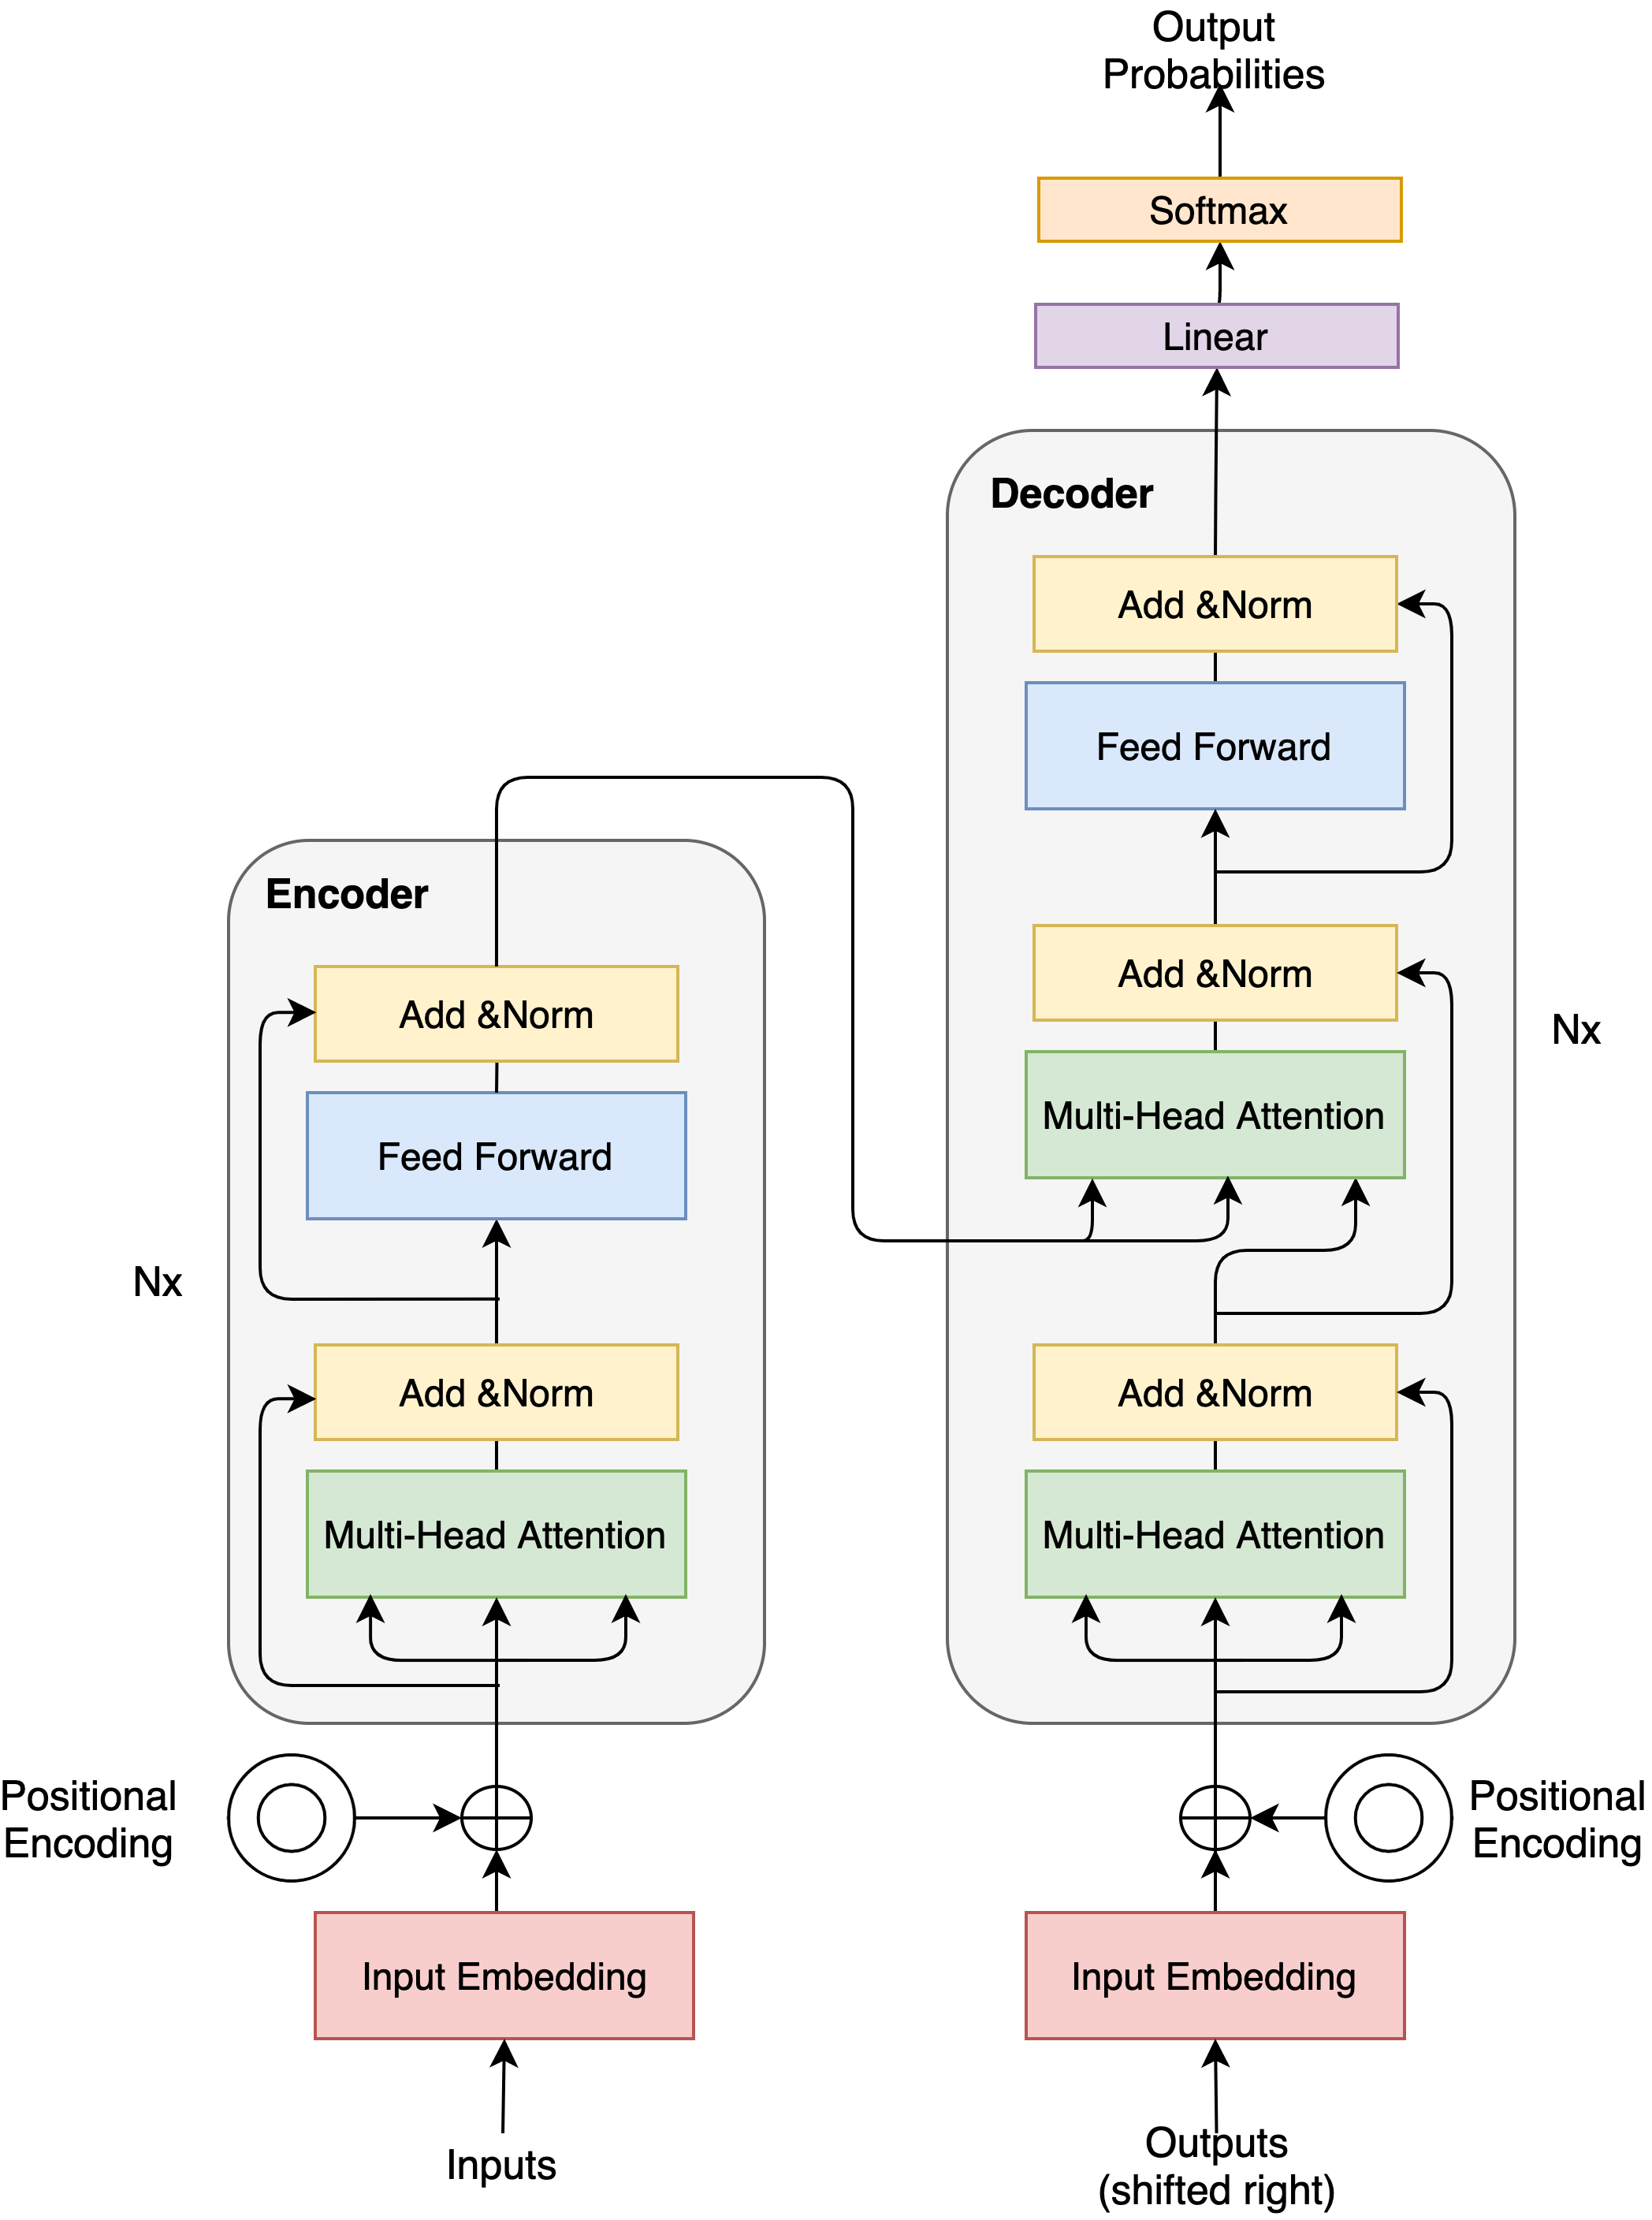
\includegraphics[width = 0.5 \textwidth]{figures/transformer.png}
	\caption[The Transformer - model architecture]
	{ The Transformer - model architecture.~\cite{vaswani2017attention}.}
	\label{fig:transformer}
\end{figure}

\subsection{Self-Attention}
An attention function can be described as mapping a query and a set of key-value pairs to an output, where the query, keys, values, and output are all vectors. The output is computed as a weighted sum of the values, where the weight assigned to each value is computed by a compatibility function of the query with the corresponding key.

From the following Table~\ref{tab:complexity_compare}, we can know that self attention has a great improvement for longer sequences. For image data, we can think of it as a longer sequence, and it would be better to optimize it.
\begin{table}[!htbp]
	\resizebox{\textwidth}{15mm}{
	\begin{tabular}{cccc}
		\hline
		Layer Type                  & Complexity per Layer & Sequential Operations & Maximum Path Length \\ \hline
		Self-Attention              & $ O(n2\cdot d)  $           &$  O(1)  $                 & $ O(1)  $               \\
		Recurrent                   & $ O(n2\cdot d) $            & $ O(n)  $                 & $ O(n)  $               \\
		Convolutional               & $O(k\cdot n\cdot d^2)$       & $O(1) $              & $O(log_k(n)$)         \\
		Self-Attention (restricted) & $ O(r\cdot  n \cdot d) $         & $ O(1)  $                 & $ O(n/r)  $             \\ \hline
	\end{tabular}}

\caption[Compare between Self-Attention and Convolutional ]
{ Maximum path lengths, per layer complexity and minimum number of sequential operations for different layer types. n is the sequence length, d is the representation dimension, k is the kernel size of convolutions and r the size of the neighborhood in restricted self-attention. Obtained from ~\cite{vaswani2017attention}.}
	\label{tab:complexity_compare}
\end{table}

There are three very important vectors in attention, query, key, and value. For self-attention, these three vectors are obtained by multiplying the same vector by different matrices (see Fig.~\ref{fig:attention}).An attention function can be described as mapping a query and a set of key-value pairs to an output. The input consists of queries and keys of dimension $ d  $, and values of dimension $ d $, the softmax function to obtain the weights on the values.


\begin{equation}
	Attention(Q,K,V)=softmax(\frac{QK^T}{\sqrt{d_K}})V
	\label{equ:self_attention}
\end{equation}


\begin{figure}[!htbp]
	\centering
	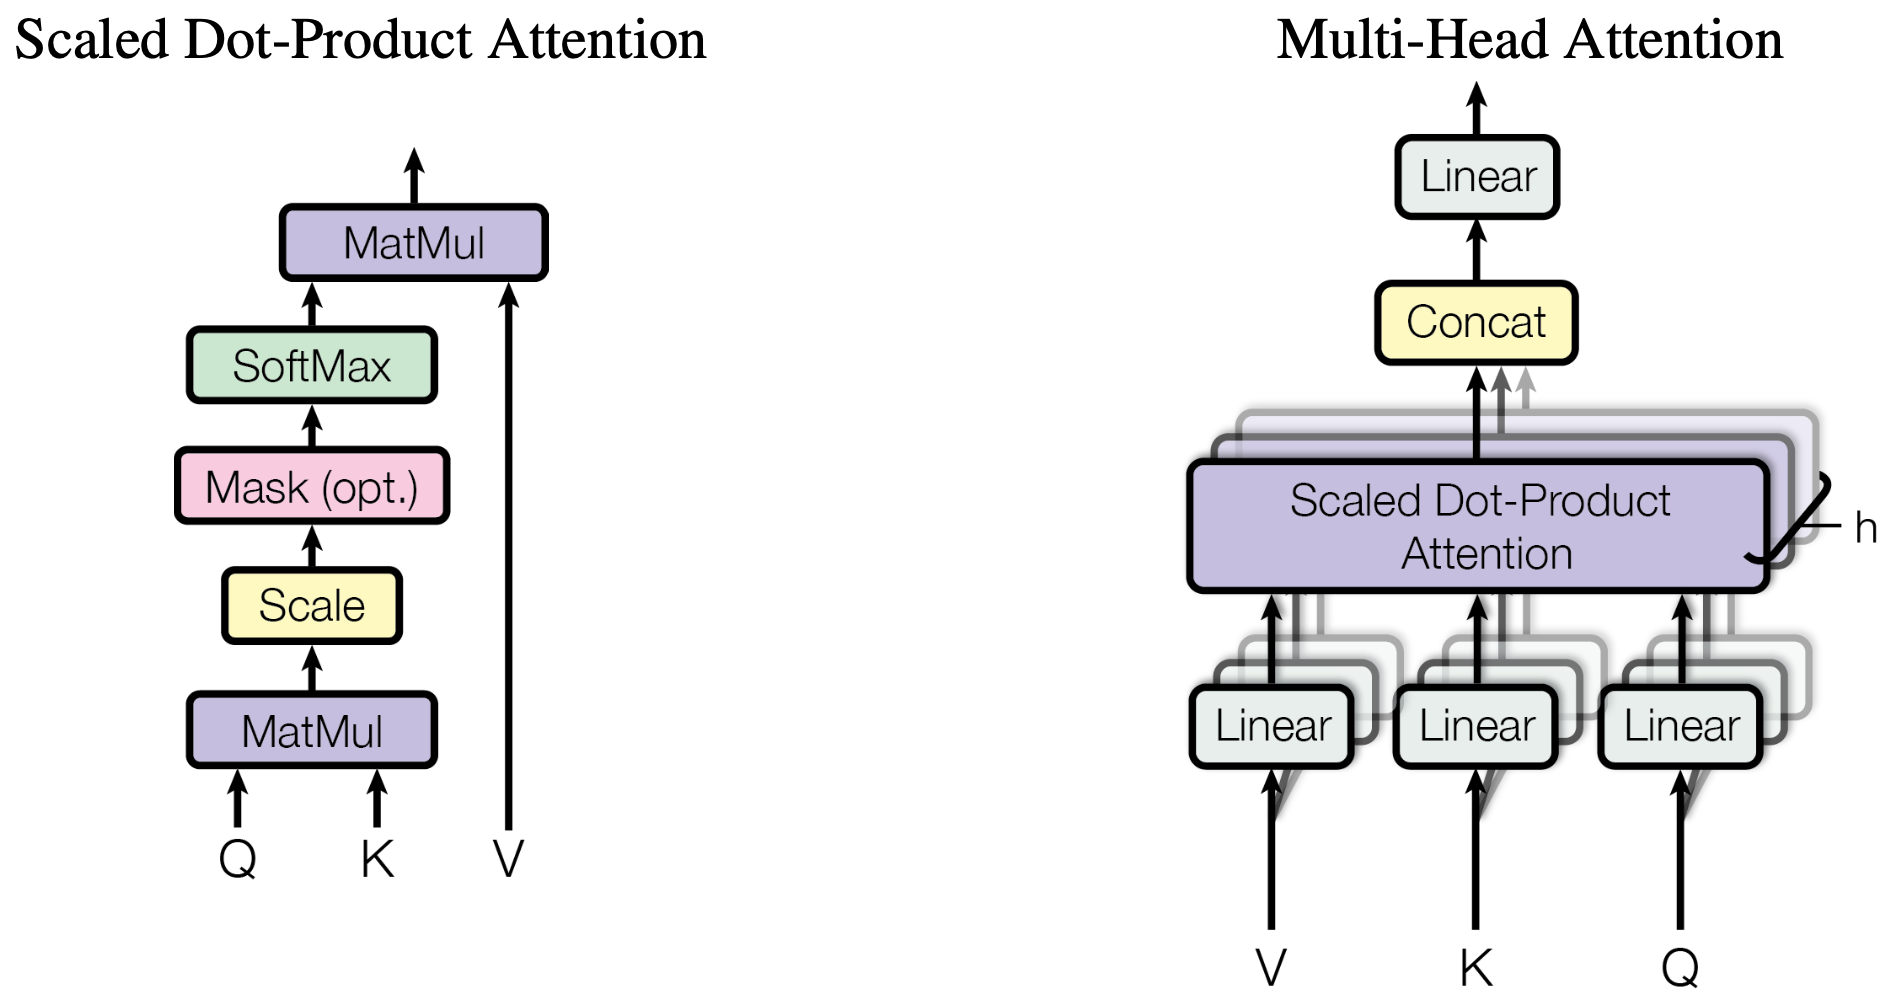
\includegraphics[width = 0.8\textwidth]{figures/attention.png}
	\caption[Scaled Dot-Product Attention and Multi-Head Attention]
	{ (left) Scaled Dot-Product Attention. (right) Multi-Head Attention consists of several attention layers running in parallel. (Image source:~\cite{vaswani2017attention}).}
	\label{fig:attention}
\end{figure}

\subsection{Multihead Attention}

Multi-head attention allows the model to attend to different representation subspaces at different positions and therefore process richer information. The queries, keys and values are linearly projected h times with different, learned linear projections to $ dk $, $ dk $ and $ dv $ dimensions respectively. On each of these projections the attention function is computed in parallel, resulting in dv dimensional output values. These are concatenated and projected to obtain the final values, as depicted in Figure 2.3.

\begin{equation}
	\begin{aligned}
MultiHead(Q,K,V) = Concat(head_1,...,head_h)W^O, \\
where \ head_i = Attention(QW_i^Q,KW_i^K,VW_i^V)
\end{aligned}
\end{equation}

\subsection{Positional Encoding}
In the case of RNNs, we feed the words sequentially to the model, each token is aware of how it was ordered. However, multi-head attention computes the output of each item in the sequence independently with no notion of word order. It is inefficient to model the sequence information without any special order or position. To account for the order of the words in the input sequence, the Transformer model adds a vector to each input embedding called Positional Encoding. Positional Encoding from the Transformer model is computed by sine and cosine functions of different frequencies as:
\begin{equation}
	\begin{aligned}
	PE_{(pos,2i)} = sin(pos/10000^{2i/d_{model}}),\\
	PE_{(pos,2i+1)} = cos(pos/10000^{2i/d_{model}})
	\end{aligned}
	\label{equ:position_embedding}
\end{equation}

\subsection{Encoder-Decoder Architecture}
The Transformer model with its encoder and decoder components is illustrated in Figure 11. Both Encoder and Decoder are composed of multiple identical encoders and decoders that can be stacked on top of each other Nx times. The encoder stack and the decoder stack share the same number of Nx.

\textbf{Encoder}: The encoder block is a stack of Nx identical layers. Each layer has a multi-head self-attention mechanism sub-layer followed by a position-wise fully connected feed-forward network sub-layer. There are two on each floor sub-layer, the first is a multi-head self-attention mechanism, and the second is a simple feed-forward network with fully connected locations. The residual structure ~\cite{He_2016_CVPR} (see figure ~\ref{fig:transformer})is used on both sub-layers, and finally layer normalization ~\cite{ba2016layer}. That is, the output of each sub-layer is $LayerNorm(x + Sublayer(x))$, where $Sublayer(x)$ is the function implemented by the sub-layer itself. Since the model does not contain any recurrence and convolution, an embedding must be added to the input so that the model can be used in order of the sequence.

The input received by an encoder is a list of vectors, it will input the list of vectors to the self-attention layer, then pass through the feed-forward neural network layer(FFN), and finally get the output, which is passed to the next encoder. The word at each position passes through the self-attention layer, and each output vector obtained passes through the FFN separately, and the feed-forward neural network through each vector is the same.


\textbf{Decoder}: The decoder block is also a stack of Nx identical layers. In addition to the two sub-layers in each encoder layer, the decoder has an extra Masked Multi-Head Attention sub-layer to avoid this attention sub-layer looking into the future.


\section{Faster R-CNN}

Faster R-CNN~\cite{ren2016faster} is an advanced network for object detection and the cornerstone for the visual relationship detection models. Compared with other object detection models, Faster R-CNN performs well on localizing and classifying the objects in images. Therefore, it is used as the backbone of object detection in many works about visual relationship detection~\cite{zellers2018neural}. Faster R-CNN contains four parts: convolutional layers, region proposal network (RPN), ROI pooling and classifier. In visual relationship detection, the first three parts are utilized to extract the feature map and localize the bounding boxes of objects. The classifier of Faster R-CNN is generally replaced by the advanced model which is designed for visual relationship detection. The structure of Faster R-CNN is illustrated in Fig.~\ref{fig:fasterrcnn}.

\begin{figure}[!htbp]
	\centering
	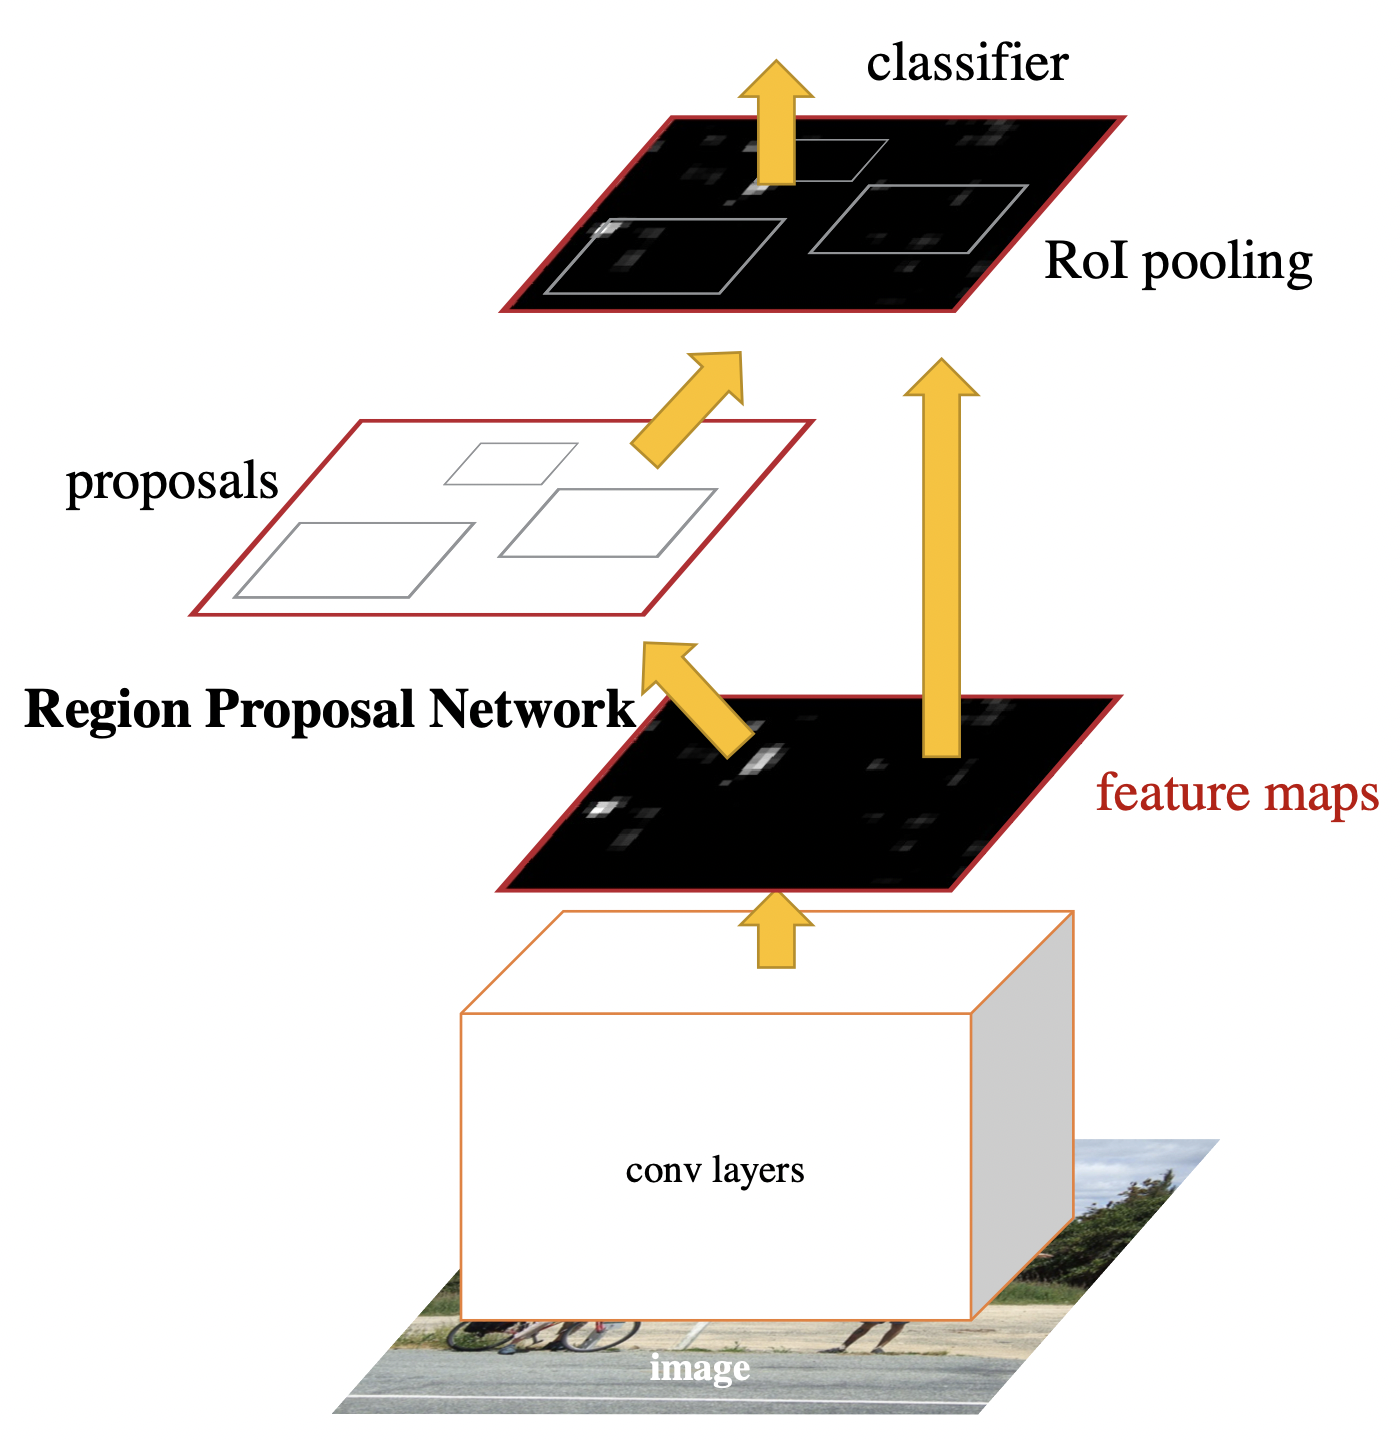
\includegraphics[width = 0.7\textwidth]{figures/fasterrcnn.png}
	\caption[The architecture of Faster R-CNN]
	{ The architecture of Faster R-CNN.}
	\label{fig:fasterrcnn}
\end{figure}

The following are the key steps of Faster RCNN:
\begin{itemize}
	\item \textbf{Conv layers.} As a CNN network target detection method, Faster R-CNN first uses a set of basic conv, relu and pooling layers to extract image feature maps. The feature maps are shared for the subsequent RPN layer and fully connected layer.
	\item \textbf{Region Proposal Networks.} The RPN network is used to generate region proposals. This layer judges that anchors belong to foreground or background through softmax, and then uses bounding box regression to correct anchors to obtain accurate proposals.
	\item \textbf{Roi Pooling. }This layer collects the input feature maps and proposals, extracts the proposal feature maps after synthesizing the information, and sends them to the subsequent fully connected layer to determine the target category.
	\item \textbf{Classification}. Use proposal feature maps to calculate the category of the proposal, and again bounding box regression to obtain the final precise position of the bounding box.
\end{itemize}

\subsection{VGG16}

VGG16 is a convolutional neural network model proposed by K. Simonyan and A. Zisserman from the University of Oxford in the paper ``Very Deep Convolutional Networks for Large-Scale Image Recognition''~\cite{simonyan2015deep}. The model achieves 92.7\% top-5 test accuracy in ImageNet~\cite{ILSVRC15}, which is a dataset of over 14 million images belonging to 1000 classes.

The structure of VGG16 is shown in Fig.~\ref{fig:vgg16}.The input to cov1 layer is of fixed size 224 x 224 RGB image. The image is passed through a stack of convolutional (conv.) layers, where the filters were used with a very small receptive field: 3x3 (which is the smallest size to capture the notion of left/right, up/down, center). In one of the configurations, it also utilizes 1x1 convolution filters, which can be seen as a linear transformation of the input channels (followed by non-linearity). The convolution stride is fixed to 1 pixel; the spatial padding of conv. layer input is such that the spatial resolution is preserved after convolution, i.e. the padding is 1-pixel for 3x3 conv. layers. Spatial pooling is carried out by five max-pooling layers, which follow some of the conv.  layers (not all the conv. layers are followed by max-pooling). Max-pooling is performed over a 2x2 pixel window, with stride 2.

Three Fully-Connected (FC) layers follow a stack of convolutional layers (which has a different depth in different architectures): the first two have 4096 channels each, the third performs 1000-way ILSVRC classification and thus contains 1000 channels (one for each class). The final layer is the soft-max layer. The configuration of the fully connected layers is the same in all networks.

All hidden layers are equipped with the rectification (ReLU) non-linearity. It is also noted that none of the networks (except for one) contain Local Response Normalisation (LRN), such normalization does not improve the performance on the ILSVRC dataset, but leads to increased memory consumption and computation time.


\begin{figure}[!htbp]
	\centering
	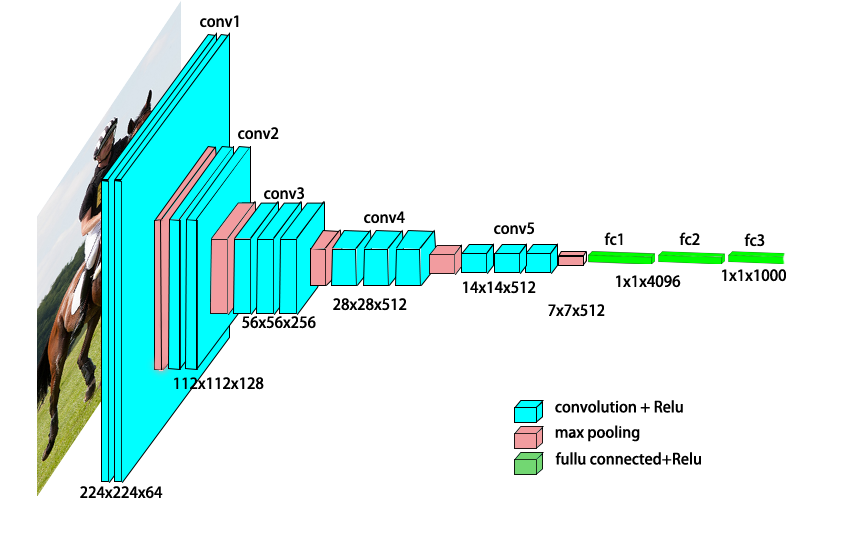
\includegraphics[width=0.8\linewidth]{figures/vgg16}
	\caption[The Architecture of VGG-16]{The Architecture of VGG-16.}
	\label{fig:vgg16}
\end{figure}

The advantages of VGG:
\begin{itemize}
	\item The structure of VGGNet is very simple, the entire network uses the same size of the convolution kernel size (3x3) and maximum pooling size (2x2).
	\item The combination of several small filter (3x3) convolutional layers is better than a large filter (5x5 or 7x7) convolutional layer.
	\item It is verified that performance can be improved by continuously deepening the network structure.
\end{itemize}

The disadvantages of VGG:

\begin{itemize}
	\item VGG consumes more computing resources and uses more parameters, resulting in more memory usage. Most of the parameters are from the first fully connected layer. VGG has 3 fully connected layers.
\end{itemize}



\label{sec:roialign}
\subsection{ROI Align}
ROI Align is a regional feature aggregation method proposed in the Mask-RCNN~\cite{he2018mask} paper, which solves the problem of regional mis-alignment caused by two quantizations in the ROI Pooling operation. Experiments show that replacing ROI Pooling with ROI Align in the detection task can improve the accuracy of the detection model.

\begin{figure}[!htbp]
	\centering
	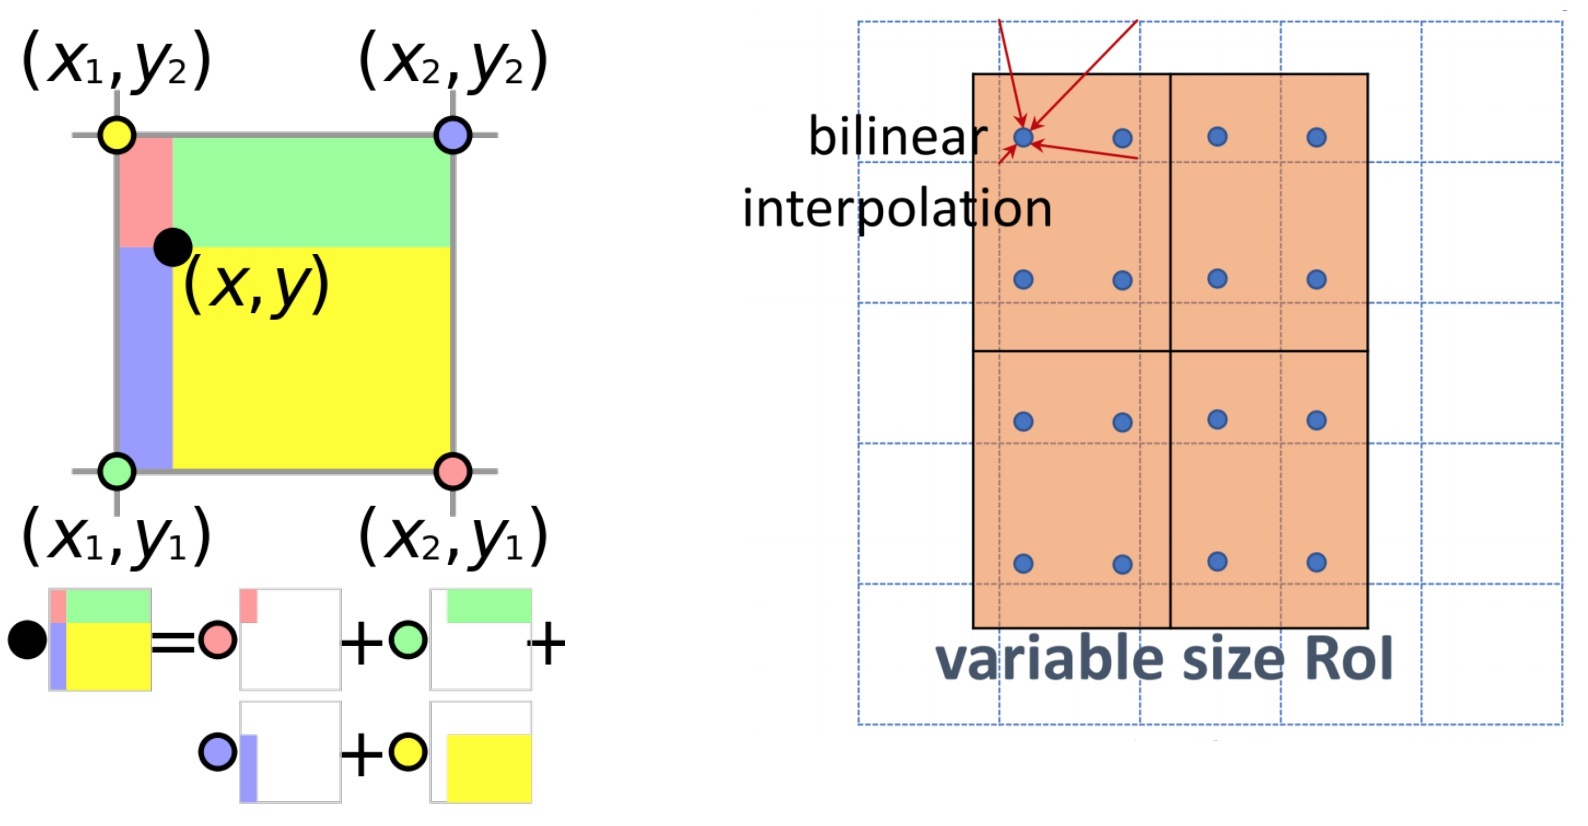
\includegraphics[width=1\linewidth]{figures/roi_align}
	\caption[Bilinear interpolation for ROI Align]{Bilinear interpolation for ROI Align.}
	\label{fig:roialign}
\end{figure}

ROI Align does not need to perform rounding operations like ROI pooling. If the decimal number is calculated, that is, it does not fall on the real pixel, then use the nearest pixel to perform bilinear interpolation on this virtual pixel to get this `pixel'  value.The step are processed as follow:

\begin{enumerate}[1.]
	\item Divide the bbox area into equal parts according to the size required by the output. It is likely that the vertices will not fall on the real pixels after the equal division.
	\item If the vertices do not fall on the real pixel points after equal division, then take a fixed 4 points in each bin, which is the blue point on the right side of Figure~\ref{fig:roialign}.
	\item For each blue point, the value of the 4 nearest real pixel points is weighted (bilinear interpolation) to obtain the value of this blue point.
	\item  Four new values are calculated in a bin, and max is selected from these new values as the output value of this bin Therefore we use bilinear interpolation to predict its value.
	\item Get the final 2x2 output.
\end{enumerate}

\section{End-to-End Object Detection with Transformers}
The DETR discards the traditional Faster R-CNN ROI-based object detection method, and uses Transformer and its proposed bipartite matching to achieve position-independent and unique bounding box for each object, thus eliminating the need for Anchor and NMS. With a very simple architecture, it achieves an accuracy comparable to or even surpassing Faster R-CNN. While being able to do object detection, the model also has better migration capabilities. In the original paper, the panoramic segmentation was achieved through the Transformer's Attention mechanism. 

\begin{figure}[!htbp]
	\centering
	\includegraphics[width = 1 \textwidth]{figures/DETR.png}
	\caption[The framework of DETR model]
	{ The framework of DETR model. Figure obtained from ~\cite{carion2020end}.}
	\label{fig:detr}
\end{figure}

The network structure of DETR is very simple (see Fig.~\ref{fig:detr}.). It is divided into three parts: the first part is a traditional CNN to extract image features to higher dimensions. The second part is a Transformer Encoder and Decoder to extract the object features. Finally, the Bipartite matching loss is used to Train the network. 

\subsection{Transformer Encoder}

As shown on the left side of the Fig.~\ref{fig:detr}, the DETR first enter the picture $ x_{img} \in  \mathbb{R} ^{3\times H_0\times W_0} $. After processing by CNN backbone, output feature map $ f \in \mathbb{R} ^{C\times H\times W } $, where $ C = 2048, H=\frac{H_0}{32}, W=\frac{W_0}{32}  $. Then add the feature map and position encoding, and input them into the Transformer Encoder for processing, and obtain the image embedding for input to the Transformer Decoder. Since the input of Transformer is serialized data, the feature map output by backbone is further processed and converted into serialized data. 
As shown on the left side of the figure, the result of detr's transformer encoder is the same as the traditional transformer structure, except that the input is replaced with image features.

\subsection{Transformer Decoder}

detr passes the predicted target sequence obtained by the Transformer encoder through the Transformer decoder shown in the right half of Figure~\ref{fig:detrtr}, and decodes it in parallel to obtain the output sequence (rather than outputting it element by element like machine translation). Different from the traditional autogreesive mechanism, each layer can decode N targets. Due to the position invariance of the decoder, that is, the result of switching the input order is unchanged, in addition to the information of each pixel itself, the position information is also very important, so these N targets The input embedding must be different to produce different results, so learn the method in NLP, add positional encoding and add it for each layer.

In addition, a fixed-size learnable object query is designed in DETR, which defines an embedding layer with a size of $ [100, 256] $, and uses its parameters as the object query. While training the network, the object query is also training, so that the most suitable query tensor is obtained and fixed.

\begin{figure}
	\centering
	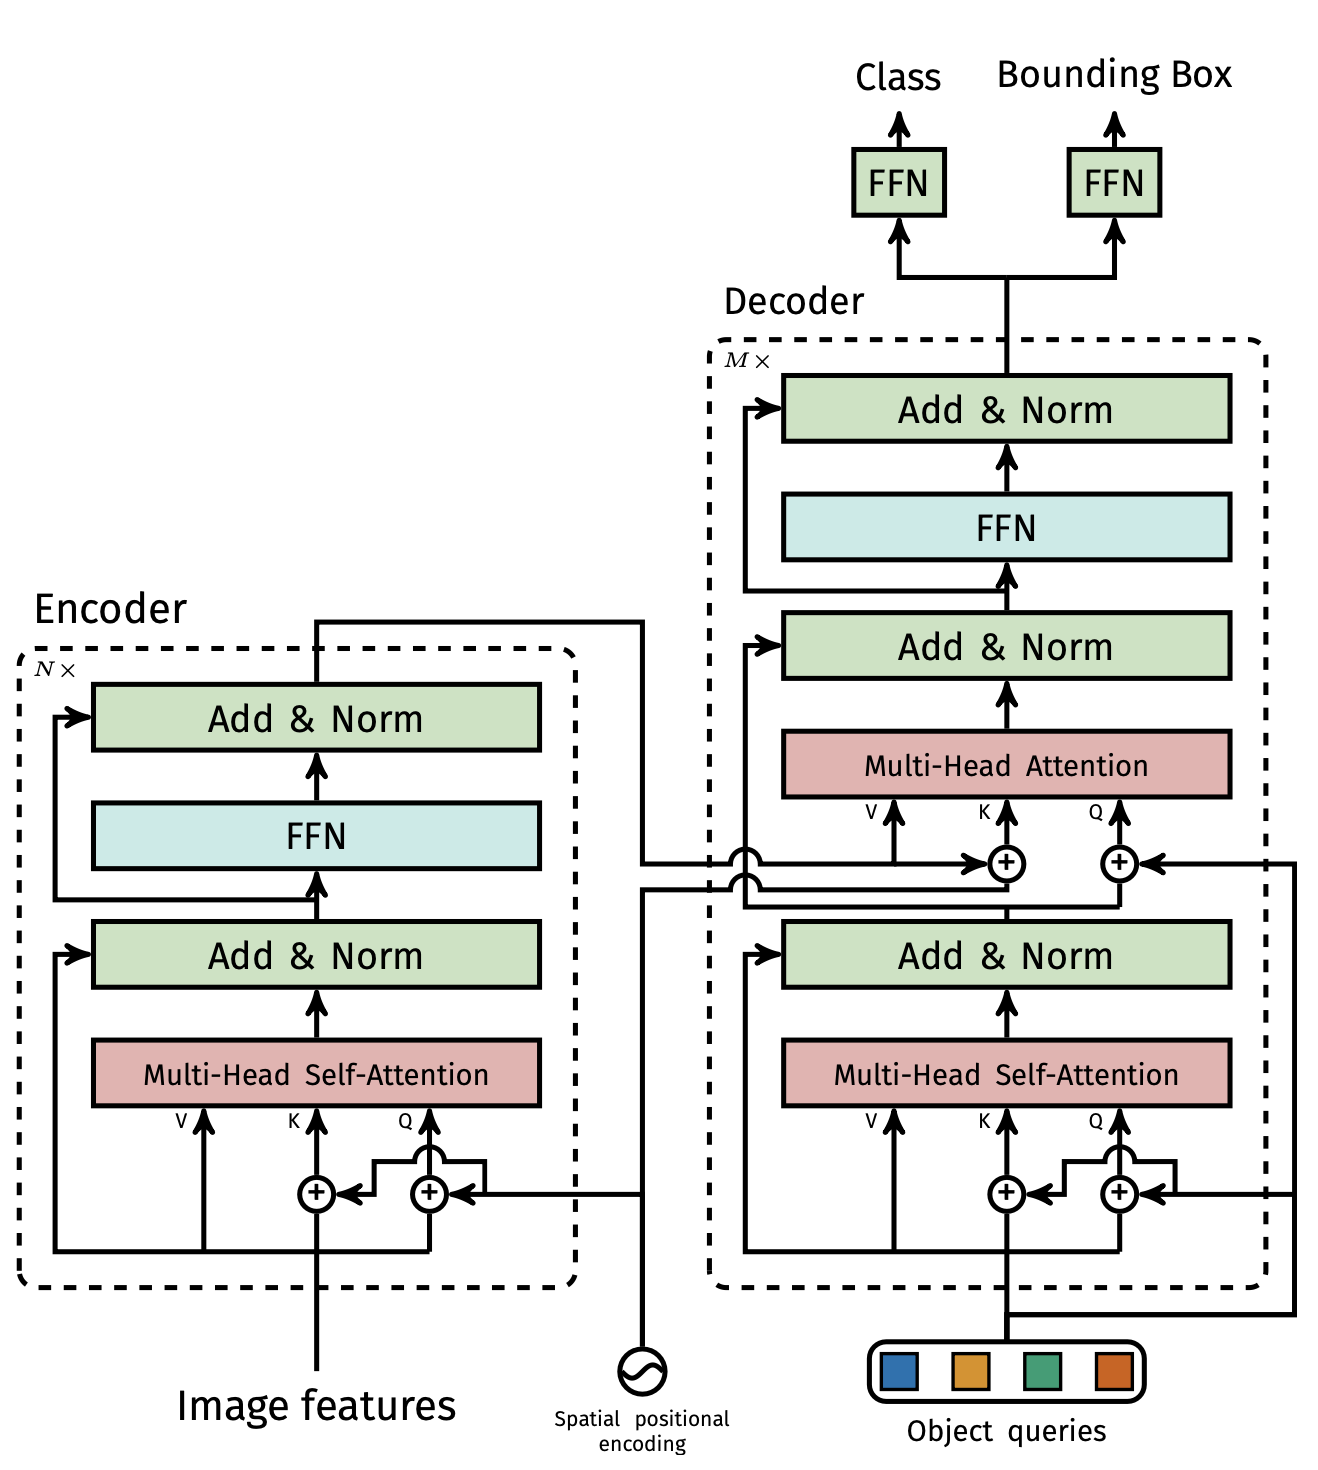
\includegraphics[width=0.7\linewidth]{figures/detr_tr}
	\caption[Architecture of DETR's transformer]{Architecture of DETR's transformer, figture obtained from ~\cite{carion2020end}.}
	\label{fig:detrtr}
\end{figure}


\subsection{Bipartite matching loss}
\label{sec:matchingloss}
Previously, the detector used the anchor and ground truth IoU to determine the positive and negative samples,  while DETR used bipartite matching loss to determine the positive and negative samples. 

\begin{equation}
	\hat{\sigma}=\underset{\sigma \in \mathfrak{G}_{N}}{\arg \min } \sum_{i}^{N} \mathcal{L}_{\text {match }}\left(y_{i}, \hat{y}_{\sigma(i)}\right)
\end{equation}

where $ \mathcal{L}_{\text {match }} $ is the pair-wise matching cost between ground true and predicted bounding boxes. Through one-by-one pairing, there is no need to adopt traditional NMS, because a bounding box can only be matched with a ground true, which will inevitably introduce loss. The algorithm implementation uses the Hungarian algorithm.

DETR obtain the predicted distributions of classes and bounding boxes through two different feed forward networks(FFN). Let us denote by $ y $ the ground truth set of objects, and $  \hat{y}= \{ \hat{y}_i\} ^N_{i=1} $ the set of $ N  $predictions.To find a bipartite matching between these two sets we search for a permutation of $ N $ elements $sigma \in \Theta _N $ with the lowest cost:
\begin{equation}\label{equ:matcher}
	\hat{\sigma} = \underset{\sigma \in \Theta _N }{argmin} \sum_{i}^{N} \mathcal L_{match} (y_i,\hat{y}_{\sigma(i)})
\end{equation}

where $\mathcal L_{match} (y_i,\hat{y}_{\sigma(i)})$ is a pair-wise matching cost between ground truth $ y_i $ and a prediction with index $ \sigma(i) $.

Then we use the \textit{Hungarian loss }in DETR~\cite{carion2020end} to calculate the loss function:
\begin{equation}\label{equ:hungarianloss}
	\begin{aligned}
		&\mathcal L_{Hungarian}(y,\hat{y} ) = \sum^{N}_{i=1}[-\log{\hat{p}_{\hat{\sigma}(i)}(c_i)} + \mathbb{I}_{\{c_i \ne  \varnothing \}}\mathcal{L}_{box}(b_i,\hat{b}_{\hat{\sigma}(i)})   ], \\
		&wehre \\
		&\mathcal{L}_{box}(b_i,\hat{b}_{\hat{\sigma}(i)}) = \lambda_{iou}\mathcal{L}(b_i,\hat{b}_{\sigma(i)}) + \lambda_{L1}\left \| b_i - \hat{b}_{\sigma (i)}  \right \| _1
	\end{aligned}
\end{equation}

where $ \hat{\sigma} $ is the optimal assignment computed in the Equ.~\ref{equ:matcher}. we define probability of class $ c_i $ as $ \hat{p}_{\hat{\sigma}(i)}(c_i)$ and the predicted box as $ \hat{b}_{\sigma(i)} $. we use a linear combination of a negative log-likelihood for class prediction and a linear combination of the $  l_1  $ loss and the generalized IoU~\cite{rezatofighi2019generalized} loss for the box prediction.

\subsubsection{Hungarian matching }

Hungarian matching is binary matching using the Hungarian algorithm, it is also a maximum matching. The purpose of maximum matching is to match an edge for each node as much as possible, and the match with the largest number of edges is the maximum match. Usually, in binary matching, each node can only match one edge.

\begin{figure}
	\centering
	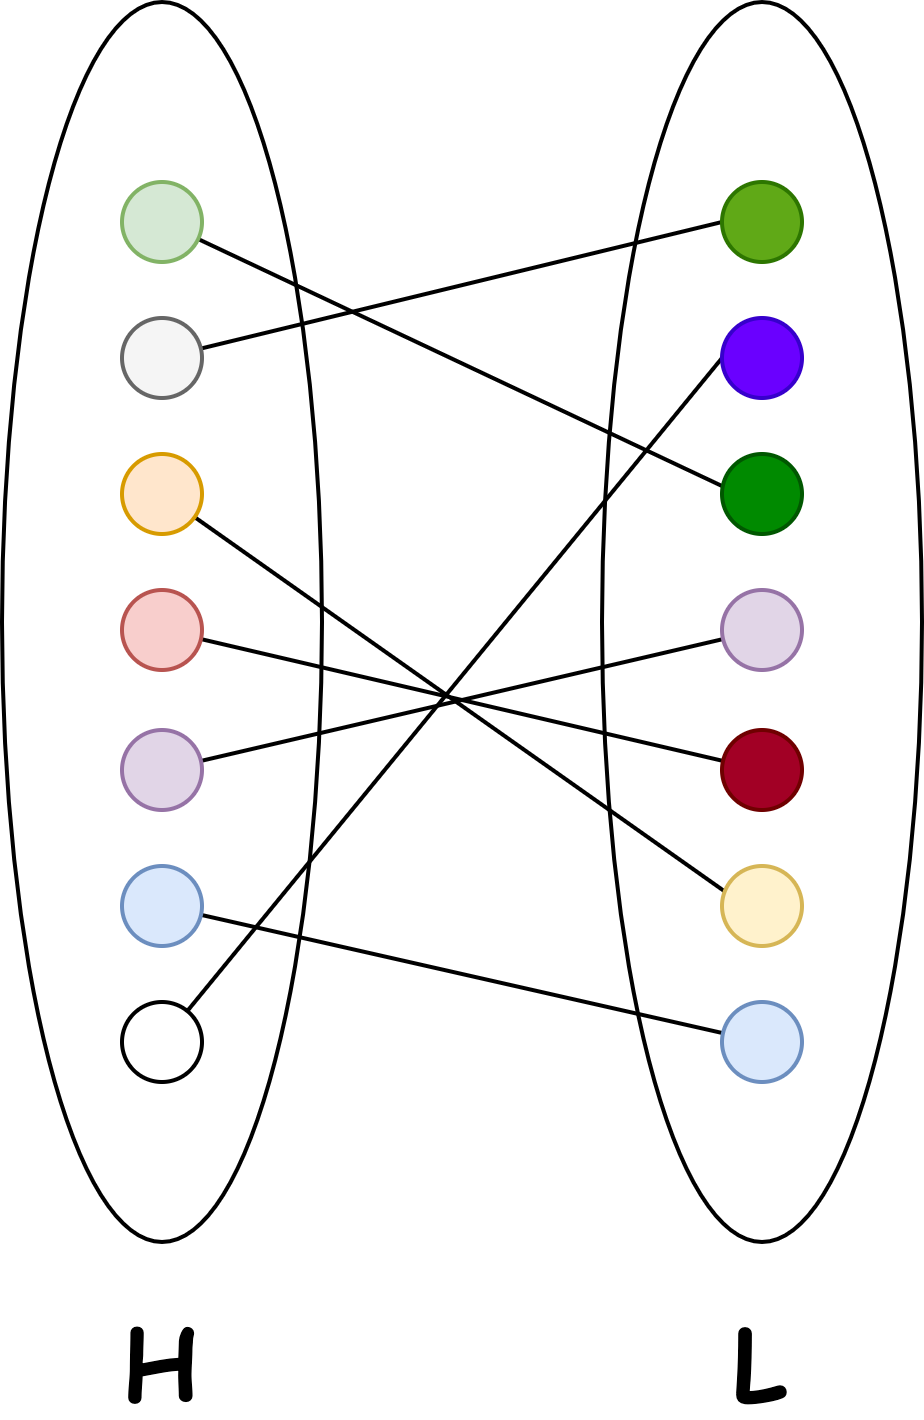
\includegraphics[width=0.3\linewidth]{figures/matcher}
	\caption[Bipartite matching loss]{Bipartite matching loss.}
	\label{fig:matcher}
\end{figure}

The basic steps of the Hungarian algorithm are as follows:
\begin{enumerate}[1.]
	\item Subtract the smallest entry in each row from all the other entries in the row. This will make the smallest entry in the row now equal to 0.
	\item Subtract the smallest entry in each column from all the other entries in the column. This will make the smallest entry in the column now equal to 0.
	\item Draw lines through the row and columns that have the 0 entries such that the fewest lines possible are drawn.
	\item  If there are nn lines drawn, an optimal assignment of zeros is possible and the algorithm is finished. If the number of lines is less than nn, then the optimal number of zeroes is not yet reached, then go to the next step.
	\item Find the smallest entry not covered by any line. Subtract this entry from each row that is not  crossed out, and then add it to each column that is crossed out. Then, go back to $ 3^{rd} $Step.
\end{enumerate}




\subsubsection{IoU and GIoU}

IoU is what we call cross-union ratio, which is the most commonly used index in target detection, in the anchor-based method. The function is not only used to determine the positive sample and the negative sample, but also can be used to evaluate the distance between the predict box and the ground-truth.

$$
I o U=\frac{|A \cap B|}{|A \cup B|}
$$

GIoU was proposed by Hamid et al.~\cite{rezatofighi2019generalized}, since IoU is the concept of ratio, it is not sensitive to the scale of the target object. However, the BBox regression loss (MSE loss, $ l_1 $ smooth loss, etc.) optimization and IoU optimization in the detection task are not completely equivalent, and the Ln norm is also sensitive to the scale of the object, and IoU cannot directly optimize the part that does not overlap.
$$
G I o U=I o U-\frac{\left|A_{c}-U\right|}{\left|A_{c}\right|}
$$

The above formula means: first calculate the area of the smallest closed area of the two boxes, that is, the area of the smallest box that contains both the predicted box and the ground truth box, then calculate the IoU, and then calculate the area of the closed area that does not belong to the two boxes. The area accounts for the proportion of the closure area, and finally IoU is used to subtract this proportion to get GIoU.


\subsection{Visualizing attention}
As shown in Figure ~\ref{fig:detrattentionmap}, we can clearly see what detr pays more attention to a picture through the attention map, and the focus of each of his object features can be reflected in the attention map. Even DETR has good scalability and can be used for image segmentation.

\begin{figure}
	\centering
	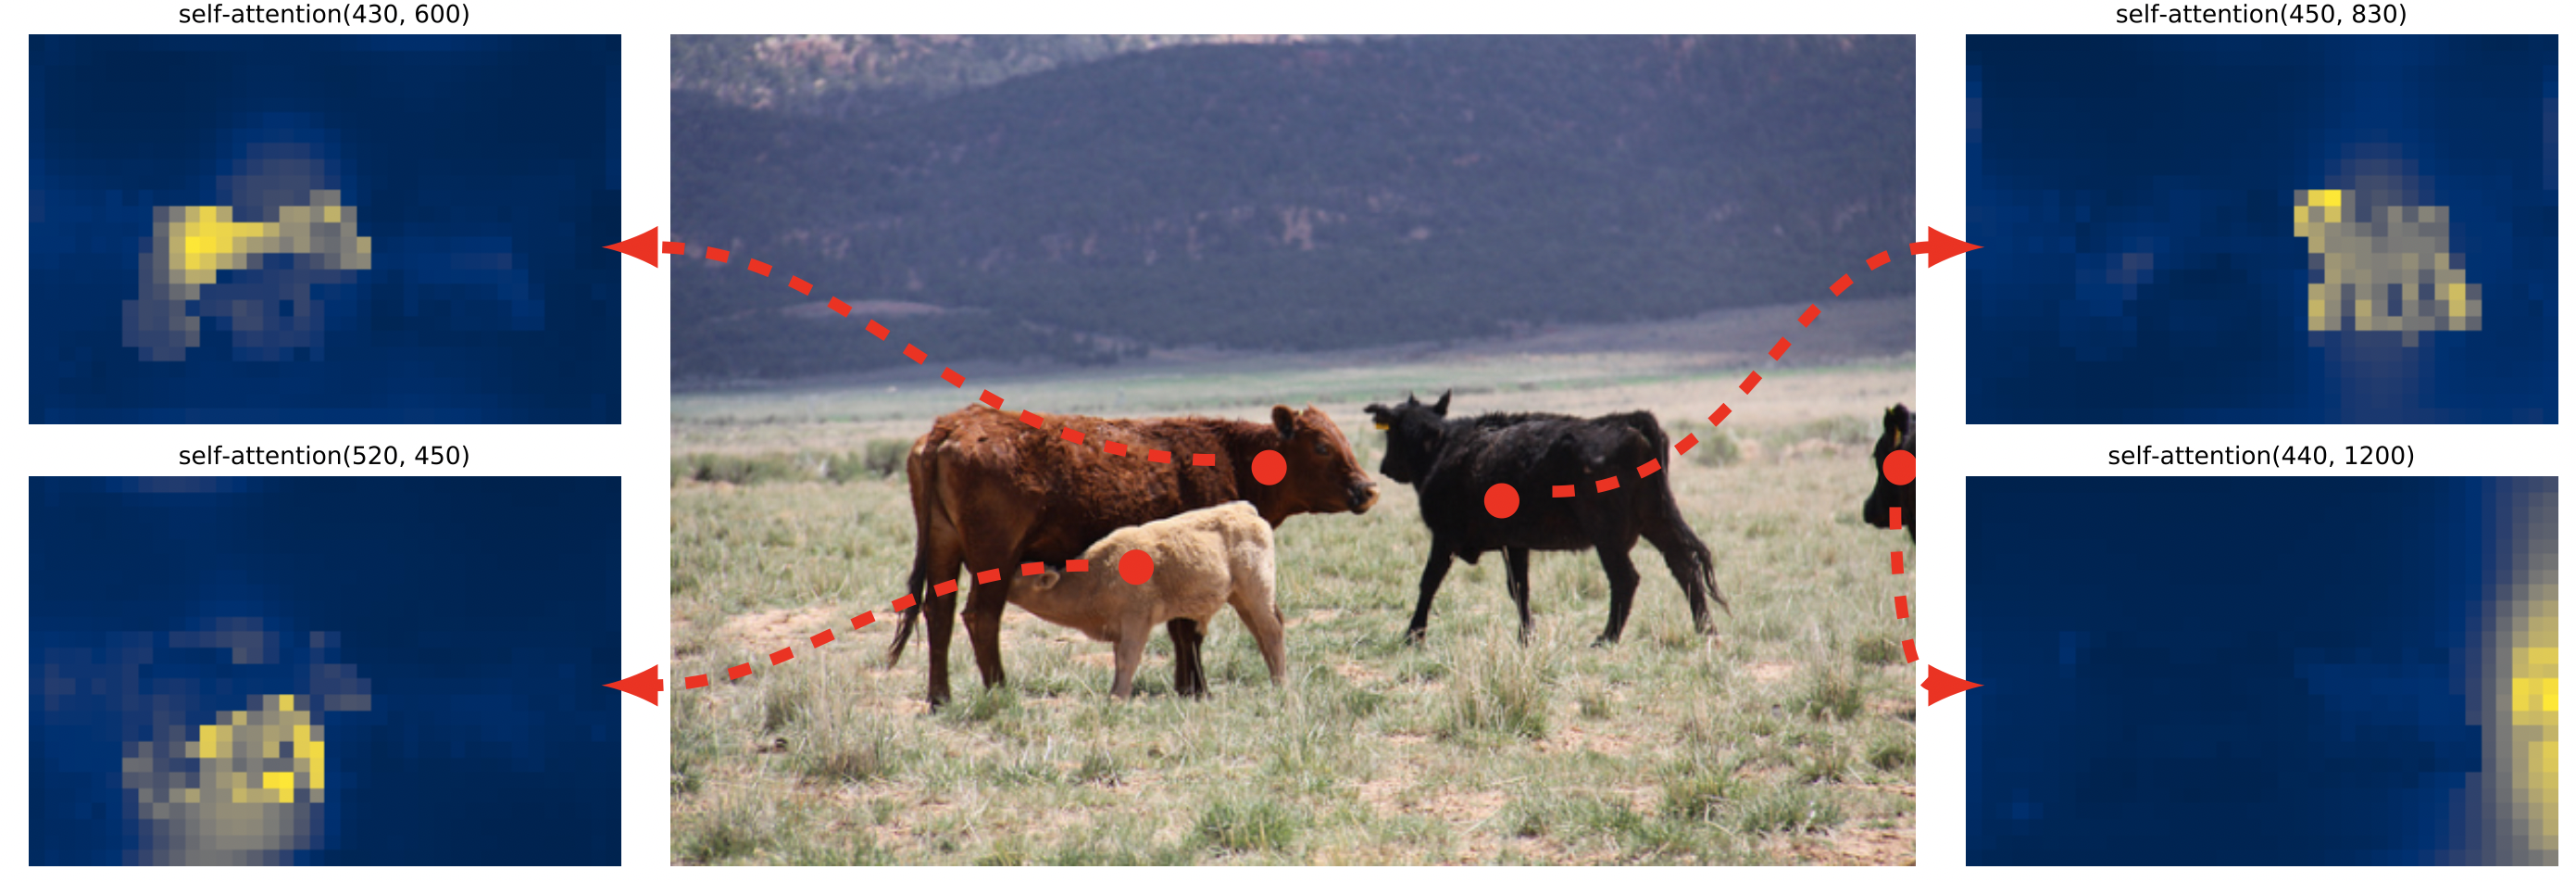
\includegraphics[width=1\linewidth]{figures/detr_attention_map}
	\caption[The attention map of the model DETR]{The attention map of the model DETR. The Encoder Self-Attention is able to separate individual instances, and it can be well visualized in the attention map. mage source from Carion et al.~\cite{carion2020end} page 11.}
	\label{fig:detrattentionmap}
\end{figure}



\label{sec:rankingloss}
\section{Ranking Loss}

Different from Cross-Entropy Loss ~\cite{Categorical_Loss} or Mean Square Error Loss(MSE) ~\cite{CHRISTOFFERSEN2004291}, their goal is to characterize the difference between the output of the model and the actual output. But ranking loss is actually a kind of metric learning, the relative distance they learn does not care about the actual value. Because there are different names in different scenes, including Contrastive Loss, Margin Loss, Hinge Loss or Triplet Loss.

Ranking loss is widely used, including two categories, such as face recognition, which is a person or not a person.

\begin{figure}[!htbp]
	\centering
	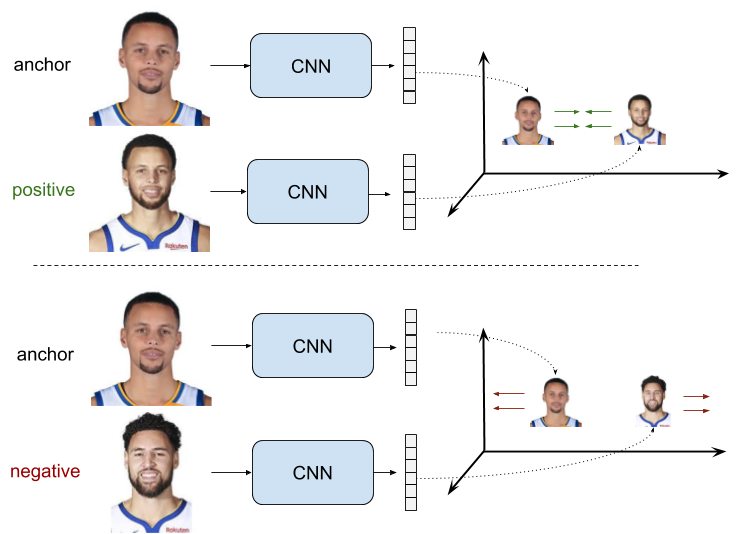
\includegraphics[width = 0.8\textwidth]{figures/pairwise_ranking_loss_faces.png}
	\caption[Example of a pairwise ranking loss ]
	{ Example of a pairwise ranking loss setup to train a net for image face verification. In this setup, the weights of the CNNs are shared. We call it siamese nets. But a pairwise ranking loss can be used in other setups, or with other nets.(Image source:~\cite{triplet_loss_em}.)}
	\label{fig:pairwise_ranking_loss}
\end{figure}


The objective is to learn representations with a small distance $d$ between them for positive pairs, and greater distance than some margin value $m$ for negative pairs. Pairwise Ranking Loss forces representations to have $0$ distance for positive pairs, and a distance greater than a margin for negative pairs. Being $r_a$ and $r_p$the samples representations and $d$ a distance function, we can write:

\begin{equation}
L=\begin{cases}
	d(r_a,r_p) & if \qquad positive\ pair \\
	max(0,m-d(r_a,r_p)) & if \qquad negative\  pair
\end{cases}
\end{equation}

Suppose $r_0,r_1 $ is used to represent the representation of the two elements of the sample, $y$is a two-valued value, when the input is a negative sample pair, it is 0, when a positive sample pair is input, it is 1, and the distance $d$ is Euclidean distance , We can have the final loss function expression:

\begin{equation}
L(r_0,r_1,y)=y\left || r_0-r_1 \right || + (1-y)max(0,m-\left || r_0-r_1 \right ||)
\end{equation}

This setup outperforms the former by using triplets of training data samples, instead of pairs. The triplets are formed by an anchor sample $x_a$, a positive sample $x_p$ and a negative sample $x_n$. The objective is that the distance between the anchor sample and the negative sample representations $d(r_a,r_n)$ is greater (and bigger than a margin $m$) than the distance between the anchor and positive representations $d(r_a,r_p)$. With the same notation, we can write:

\begin{equation}
L(r_a,r_p,r_n)=max(0,m+d(r_a,r_p)-d(r_a,r_p))
\label{equ:ranking_loss}
\end{equation}

\begin{figure}[!htbp]
	\centering
	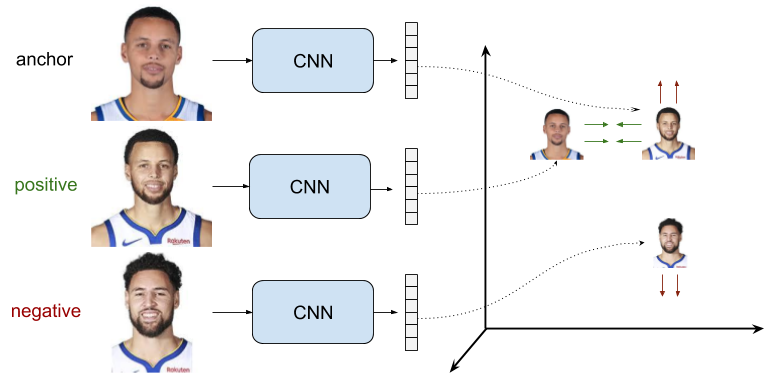
\includegraphics[width = 0.8\textwidth]{figures/triplet_loss_faces.png}
	\caption[Example of a triplet ranking loss ]
	{ Example of a triplet ranking loss setup to train a net for image face verification. In this setup, the weights of the CNNs are shared. We call it triple nets. (Image source:~\cite{triplet_loss_em}).}
	\label{fig:triplet_ranking_loss}
\end{figure}


\section{Word Representation}

Same as location information, semantic information also helps a lot for understanding relations. The basic encoding method is one hot code. 

One-hot representation is another natural approach to represent words, which assigns a unique index to each word. It is also not good enough to represent words with one-hot representation. First, one-hot representation could not capture the semantic relatedness among words. Second, one-hot representation is a high-dimensional sparse representation, which is very inefficient. Third, it is very inflexible for one-hot representation to deal with new words, which requires assigning new indexes for new words and would change the dimensions of the representation. The change may lead to some problems for existing NLP systems.

Recently, distributed word representation approaches are proposed to address the problem of one-hot word representation. The distributional hypothesis ~\cite{bojanowski2017enriching} that linguistic objects with similar distributions have similar meanings is the basis for distributed word representation learning. Based on the distributional hypothesis, various word representation models, such as CBOW and Skip-gram, have been proposed and applied in different areas.


\begin{figure}[!htbp]
	\centering
	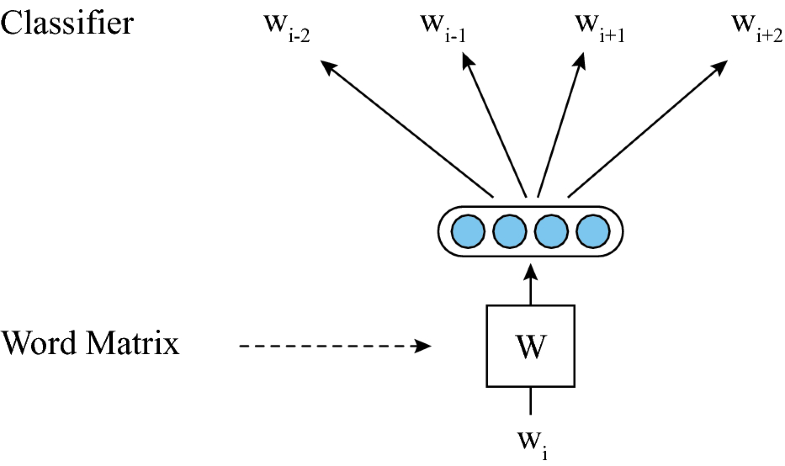
\includegraphics[width = 0.5\textwidth]{figures/skip-gram-model.png}
	\caption[The architecture of skip-gram model]
	{ The architecture of skip-gram model.}
	\label{fig:skip-gram-model}
\end{figure}

One of the widely used distributed word representation is Skip-Gram model (see Fig.~\ref{fig:skip-gram-model}) which is part of the \textbf{Word2Vec} library. It was created by a team of researchers led by Tomas Mikolov at Google. The main idea is to represent words by means of its neighbors. It tries to predict all neighboring words(the context) of a given word. According to paper~\cite{mikolov2013distributed}, the objective of model is defined as follows:$$\frac{1}{T}\sum_{t=1}^{T}\sum_{-c\le j\le c,j\ne 0} \log_{ p(w_{t+j}\mid w_t) }$$
where w is training word and c is the size of context. So its objective is to find word representations that can predict surrounding words.

Another member of distributed word representations is \textbf{Global Vectors for Word Representation(GloVe)} which is an abbreviation for Global Vectors. While Word2Vec captures certain local context window, GloVe exploits overall co-occurrence statistics of words from corpus, which is a large collection of texts. It consists of two important steps. First one constructs a matrix of term co-occurrences. For each word we compute conditional probability, e.g. for word water $ P(k\mid water) $, where $ k $ is word from vocabulary. If $ k $ is stream, the value of $ P $ is high, and if $ k $ is fashion, then expected value is low as they do not usually co-occur together. After performing all statistical computations, the large matrix is formed. Then high-dimensional context matrix is reduced by normalizing counts and log-smoothing.
